% Chapter 25 of Genesis
\bookchapter{\Abraham and \name{Keturah}}

\bverse \Abraham again took a wife\vmark{a}, and her name \was \name{Keturah}.
	\contextnote{a}{Taking multiple wives seemed to be a fairly common practice in these times.}

\bverse And she bore him \name{Zimran}, \name{Jokshan}, \name{Medan}, \name{Midian}, \name{Ishbak}, and \name{Shuah}.
\bverse \name{Jokshan} begot \name{Sheba} and \name{Dedan}. And the sons of \name{Dedan} were \name{Asshurim}, \name{Letushim}, and \name{Leummim}.
\bverse And the sons of \name{Midian} \were \name{Ephah}, \name{Epher}, \name{Hanoch}, \name{Abidah}, and \name{Eldaah}. All these \were the children of \name{Keturah}.

\begin{figure}[htbp] % h=here, t=top, b=bottom, p=page
  \centering
  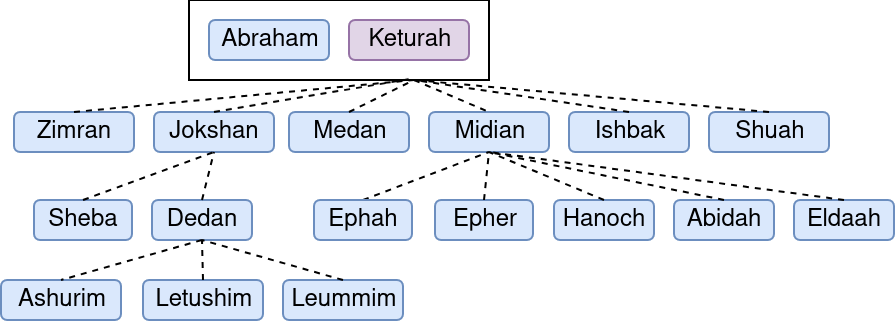
\includegraphics[width=0.8\linewidth]{images/genealogies/abraham_keturah_genealogy.png}
  \caption{This is a diagram showing the genealogy of the family of \Abraham and \name{Keturah} as outlined in \bref{Genesis 25}. Marriage is depicted with a rectangular border around the couple. This diagram was created by me using the draw.io tool \cite{draw.io}.}
  \label{fig:abraham_keturah_genealogy}
\end{figure}

\bverse And \Abraham gave all that he had to \Isaac.
\bverse But \Abraham gave gifts to the sons of the concubines which \Abraham had; and while he was still living he sent them eastward, away from \Isaac his son, to the country of the east.

\bmarkerdown{\Abraham's Death and Burial}

\bverse This \textit{is} the sum of the years of \Abraham's life which he lived: one hundred and seventy-five years.
\bverse Then \Abraham breathed his last and died in a good old age, and old man and full of \textit{years}, and was gathered to his people.
\bverse And his sons \Isaac and \name{Ishmael} buried him in the cave of \location{Machpelah}, which \textit{is} before \location{Mamre}, in the field of \name{Ephron} the son of \name{Zohar} the \people{Hittite},
\bverse the field which \Abraham purchased from the sons of \name{Heth}. There \Abraham was buried, and \Sarah his wife.
\bverse And it came to pass, after the death of \Abraham, that God blessed his son \Isaac. And \Isaac dwelt at \location{Beer Lahai Roi}.

\bmarkerdown{The Families of \name{Ishmael} and \Isaac}

\bverse Now this \textit{is} the  genealogy of \name{Ishmael}, \Abraham's son, whom \name{Hagar} the \people{Egyptian}, \Sarah's maidservant, bore to \Abraham.
\bverse And these \were the names of the sons of \name{Ishmael}, by their names, according to their generations: The firstborn of \name{Ishmael}, \name{Nebajoth}; then \name{Kedar}, \name{Abdeel}, \name{Mibsam},
\bverse \name{Mishma}, \name{Dumah}, \name{Massa},
\bverse \name{Hadar}, \name{Tema}, \name{Jetur}, \name{Naphish}, and \name{Kedemah}.

\begin{figure}[htbp] % h=here, t=top, b=bottom, p=page
  \centering
  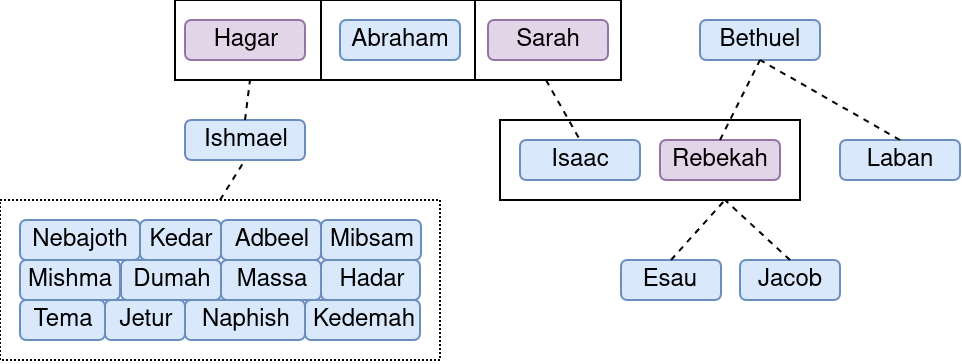
\includegraphics[width=0.8\linewidth]{images/genealogies/ishmael_isaac_genealogies.png}
  \caption{This is a diagram showing the genealogy of the family of \name{Ishmael} and \Isaac as outlined in \bref{Genesis 25}. Marriage is depicted with a rectangular border around the couple. Males are depicted in blue, while females are pink. Births are depicted as branching off from the mother. \name{Rebekah} and \name{Laban} are siblings (\bref{Genesis 25:20} and \bref{Genesis 24:29}), which likely implies \name{Laban} is \name{Bethuel}'s son (since descendants are typically tracked through the males). This diagram was created by me using the draw.io tool \cite{draw.io}.}
  \label{fig:ishmael_isaac_genealogies}
\end{figure}

\bverse These \were the sons of \name{Ishmael} and these \were their names, by their towns and their settlements, twelve princes according to their nations.
\bverse These \were the years of the life of \name{Ishmael}: one hundred and thirty-seven years; and he breathed his last and died, and was gathered to his people.
\bverse (They dwelt from \location{Havilah} as far as \location{Shur}, which is east of \location{Egypt} as you go toward \location{Assyria}.) He died in the presence of all his brethren.
\bverse This \textit{is} the genealogy of \Isaac, \Abraham's son. \Abraham begot \Isaac. 
\bverse \Isaac was forty years old when he took \Rebekah as wife, the daughter of \name{Bethuel} the \people{Syrian} of \location{Padan Aran}, the sister of \name{Laban} the \people{Syrian}.
\bverse Now \Isaac pleaded with the \lord for his wife, because she \was barren; and the \lord granted his plea, and \Rebekah his wife conceived.
\bverse But the children struggled together within her; and she said, ``If \textit{all is} well, why \textit{am} I \textit{like} this?'' So she went to inquire of the \lord.
\bverse And the \lord said to her:
\begin{bquotation}
``Two nations \are in your womb, Two peoples shall be separated from your body; \textit{One} people shall be stronger than the other, And the older shall serve the younger.''
\end{bquotation}
\bverse So when her days were fulfilled \textit{for her} to give birth, indeed \textit{there were} twins in her womb.
\bverse And the first came out red. He \was like a hairy garment all over; so they called his name \Esau\vmark{a}.
	\translationnote{a}{As stated here in context, the word `\Esau' means `hairy' \cite{Strong's GodRules}.}

\bverse Afterwards his brother came out, and his hand took hold of \Esau's heel; so his name was called \Jacob\vmark{a}. \Isaac \was sixty years old when she bore them.
	\translationnote{a}{As stated here in context, the word `\Jacob' means `heel holder' \cite{Strong's GodRules}.}

\bverse So the boys grew. And \Esau was a skillful hunter, a man of the field; but \Jacob was a mild man\vmark{a}, dwelling in tents.
	\translationnote{a}{The term `mild man' (Strong's H8535 - also often translated to `plain') implies he was a simple man - quiet, innocent, and one who does not get into trouble often. Strong's translates this word in other areas as `complete, morally innocent, having integrity' or `one who is morally and ethically pure' \cite{Strong's GodRules}.}

\bverse And \Isaac loved \Esau because he ate \textit{of his} game, but \Rebekah loved \Jacob.

\bmarkerdown{\Esau Sells His Birthright}

\bverse Now \Jacob cooked a stew; and \Esau came in from the field, and he \was faint.
\bverse And \Esau said to \Jacob, ``Please feed me with that same red \textit{stew}, for I \textit{am} faint.'' Therefore his name was called \name{Edom}\vmark{a}.
	\translationnote{a}{The name `\name{Edom}' (Strong's H123 \cite{Strong's GodRules}) means `red.' This could be because he was exhausted and red from a long time working out in the sun. Based on \bref{Genesis 25:32}, this was likely an incredibly exhausted state.}

\bverse But \Jacob said, ``Sell me your birthright as of this day.''
\bverse And \Esau said, ``Look, I \textit{am} about to die; so what \is this birthright as of this day.''
\bverse Then \Jacob said, ``Swear to me as of this day.'' So he swore to him, and sold his birthright to \Jacob.
\bverse And \Jacob gave \Esau bread and stew of lentils; then he are and drank, arose, and went his way. Thus \Esau despised his birthright\vmark{a}.
	\translationnote{a}{The term `birthright' (Strong's H1062 \cite{Strong's GodRules}) means the privilege that is given at birth. This can include an inheritance, or even leadership of a clan/family.}

